In this chapter we will lay down the general notations and definitions required for the later parts of the thesis.
In section~\ref{sec:pre:general} we will define several cryptographic primitives which are required for our constructions.
Section~\ref{sec:pre:bitcoin} will describe several definitions around Bitcoin, particularly its transaction structure.
After that in secion~\ref{sec:pre:privacy} we will discuss the notion of privacy enhancing cryptocurrencies, and then range proofs in section~\ref{sec:pre:rangeproof} of which both are needed to understand the Mimblewimble protocol discussed in section~\ref{sec:pre:mimblewimble}.
Finally we explain the concept of scriptless scripts in section~\ref{sec:pre:scriptless-scripts} and adaptor signatures~\ref{sec:pre:aptsignatures} which are both relevant building blocks for the constructions found in this thesis.

\section{General Notation and Definitions}\label{sec:pre:general}

\paragraph{Notation}
We first define the general notation used in the following chapters to formalize procedures and protocols.
Let $\cnstGroup$ denote a cyclic group of prime order $\varPrime$ and $\cnstIntegersPrime{\varPrime}$ the ring of integers modulo $\varPrime$ with identity element $\cnstIdentityElement$.
$\cnstIntegersPrimeWithoutZero{\varPrime}$ is $\cnstIntegersPrime{\varPrime} \opExcluding \funList{0}$.
$\varG \opSeperate \varH$ are adjacent generators in $\cnstGroup$, where adjacent means the discrete logarithm of $\varH$ in regards to $\varG$ is not known.
Exponentiation stands for repeated application of the group operation.
We define the group operation between two curve points as $\funGen{\varScA} \opAddPoint \funGen{\funGen{\varScB}} \opEq \funGen{\varScA \opAddScalar \varScB}$.

\begin{definition}[Hard Relation]\label{def:pre:hard-relation}
    Given a language $\varLanguage \opAssign \funList{\varBigA \opForWhich \exists\varSmallA \text{ s.t. } (\varBigA, \varSmallA) \opIn \cnstRelation}$ then the relation $\cnstRelation$ is
    considered hard if the following three properties hold:~\cite{aumayr2020bitcoinchannels}
    \begin{enumerate}
        \item $\procGenR{(\varSecParam)}$ is a $\cnstPolyTime$ sampling algorithm which outputs a statement/witness of the form $(\varBigA, \varSmallA) \opIn \cnstRelation$.
        \item Relation $\cnstRelation$ is poly-time decidable.
        \item For all $\cnstPolyTime$ adversaries $\cnstAdversary$ the probability of finding $\varSmallA$ given $\varBigA$ is negligible.
    \end{enumerate}
\end{definition}

\begin{definition}[Discrete Logarithm]\label{def:pre:discretelog}
    We define the discirte logarithm in a group $\cnstGroup$ of a number $\varN$ as the number $\varM$ such that for the groups generator $\varG$ the following holds:
    \[ \funGen{\varM} \opEqNoQ \varN \]
    The discrete logarithm is a hard relation as defined in~\ref{def:pre:hard-relation}.
\end{definition}

\begin{definition}[Signature Scheme]\label{def:pre:signature-scheme}
    A signature scheme $\varSigScheme$ is a tuple of algorithms $(\procSetupId \opSeperate \procSignId \opSeperate \procVerfId)$ defined as follows: \cite{goldwasser1988digital}
    \[ \varSigScheme = (\procSetupId \opSeperate \procSignId \opSeperate \procVerfId) \]

    \begin{itemize}
        \item $\varKeyPair \opFunResult \procSetup{\varSecParam}$: The keygen function creates a keypair $\varKeyPair$, the public key can be distributed to the verifier(s) and the secret key has to be kept private. \\
        \item $\varSignature \opFunResult \procSign{\varMsg}{\varSecKey}$: The signing function creates a signature consisting of a variable $\varS$ and $\varRand$ which is a commitment to the secret nonce $\varNonce$ used during the signing process.
        As an input it takes a message $\varMsg$ and the secret key $\varSecKey$ of the signer.
        \item $\cnstTrueorFalse \opFunResult \procVerf{\varMsg}{\varSignature}{\varPubKey}$: The verification function allows a verifier knowing the signature $\varSignature$, message $\varMsg$ and the provers public key $\varPubKey$ to verify the signatures
        validity. \\
    \end{itemize}

    A valid signature scheme has to fulfill two security properties:
    \begin{itemize}
        \item Correctness: For all messages $\varMsg$ and valid keypairs $\varKeyPair$ the following must hold with overwhealming probabillity: $\procVerf{\varPubKey}{\procSign{\varSecKey}{\varMsg}}{\varMsg} \opEq 1$
        \item Unforgeability (\cnstEUFCMA): Informally the existential unforgeability under chosen message attacks holds if an attacker $\cnstAdversary$ is unable to forge a valid signature for a chosen message.
        A formalization of the property can be found in section~\ref{subsec:sig:secureaptscheme}
    \end{itemize}
\end{definition}

\begin{definition}[Cryptographic Hash Function]\label{def:pre:hash-function}
    A cryptographic hash function $\cnstHash$ is defined as $\funHash{\varInput} \rightarrow \cnstBinary{\varN}$ for some fixed number $\varN$ and some input $\varInput$ ~\cite{al2011cryptographic}.
    A secure hashing function has to fulfill the following security properties:
    \begin{itemize}
        \item Collision-Resistence (CR): Collision-Resistance means that it is computationally infeasible to find two inputs $\varInput_1$ and $\varInput_2$ such that
        $\funHash{\varInput_1} \opAssign \funHash{\varInput_2}$ with $\varInput_1 \opNotEq \varInput_2$.
        \item Pre-image Resistence (Pre): In a hash function $\cnstHash$ that fulfills Pre-image Resistance it is infeasible to recover the original input $\varInput$ from its hash output $\funHash{\varInput}$.
        If this security property is achieved, the hash function is said to be non-invertible.
        \item 2nd Pre-image Resistence (Sec):  This property is similar to Collision-Resistance and is sometimes referred to as \textit{Weak Collision-Resistance}.
        Given such a hash function $\cnstHash$ and an input $\varInput$, it should be infeasible to find a different input $\funStar{\varInput}$ such that $\varInput \opNotEq \funStar{\varInput}$
        and $\funHash{\varInput} \opEq \funHash{\funStar{\varInput}}$.
    \end{itemize}
    The relation between the input $\varInput$ and the output $\funHash{\varInput}$ is a hard relation as defined in~\ref{def:pre:hard-relation}.
\end{definition}

\begin{definition}[Commitment Scheme]\label{def:pre:commitment}
    A cryptographic Commitment Scheme $\varCommitScheme$ is defined by a pair of functions $(\procSetupId, \procCommitId)$~\cite{bunz2018bulletproofs}.
    \begin{itemize}
        \item $\varPublicParam \opFunResult \procSetupCom{\varSecParam}$: The setup procedure is a DPT function, it takes as input a security parameter $\varSecParam$ and outputs public parameters $\varPublicParam$.
        Depending on $\varPublicParam$ we define a input space $\varInputSpace_{\varPublicParam}$, a randomness space $\varRandSpace_{\varPublicParam}$ and a commitment space $\varCommitSpace_{\varPublicParam}$.
        \item $\varCommitment \opFunResult \procCommit{\varInput}{\varNonce}$ The commit routine is DPT function that takes an arbitrary input $\varInput \opIn \varInputSpace_{\varPublicParam}$, a random value $\varNonce \opIn \varRandSpace_{\varPublicParam}$ and
        generates an output $\varCommitment \opIn \varCommitSpace_{\varPublicParam}$.
    \end{itemize}

    Secure commitments must fullfill the \emph{Binding} and \emph{Hiding} security properties:
    \begin{itemize}
        \item \textit{Binding:} If a Commitment Scheme is binding it must hold that for all $\cnstPolyTime$ adversaries $\cnstAdversary$ given a valid input $\varInput \opIn \varInputSpace_{\varPublicParam}$
        and randomness $\varNonce \opIn \varRandSpace_{\varPublicParam}$ the probabilty of finding a $\funStar{\varInput} \opNotEq \varInput$ and a $\funStar{\varNonce}$ with
        $\procCommit{\varInput}{\varNonce} \opEqNoQ \procCommit{\funStar{\varInput}}{\funStar{\varNonce}}$ is negligible.
        \item \textit{Hiding:} For a $\cnstPolyTime$ adversary $\cnstAdversary$, commitment inputs $\varInput_0, \varInput_1 \opIn \varInputSpace_{\varPublicParam}$ randomness $\varNonce \opIn
       \varRandSpace_{\varPublicParam}$ and a commitment output $\varCommitment \opAssign \procCommit{\varInput_{\varB}, \varNonce}$ the probabilty of the adversary choosing the correct $\varB$ out of $\{0,1\}$
        must not be higher then $\frac{1}{2} + \funNegl{\varProbability}$.
    \end{itemize}
\end{definition}

\begin{definition}[Additive Homomorphic Commitment]\label{def:pre:homo-com}
    A Commitment Scheme as defined in~\ref{def:pre:commitment} is said to be addtive homomorphic if the following holds~\cite{bunz2018bulletproofs}
    \[ \procCommit{\varInput_1}{\varNonce_1} \opAddPoint \procCommit{\varInput_2}{\varNonce_2} \opEqNoQ \procCommit{\varInput_1 \opAddScalar \varInput_2}{\varNonce_1 \opAddScalar \varNonce_2} \]
\end{definition}

\begin{definition}[Pedersen Commitment Scheme]\label{def:pre:pedersen}
    A \emph{Pedersen Commitment Scheme} is an instance of a Commitment Scheme as defined in definition~\ref{def:pre:commitment} that has the additive homomorphic property as defined in~\ref{def:pre:homo-com}.

This can be achieved as follows:
    $\varCommitSpace_{\varPublicParam} \opAssign \cnstGroup$ of order $\varPrime \opSeperate \varInputSpace_{\varPublicParam} \opSeperate \varRandSpace_{\varPublicParam} \opAssign \cnstIntegersPrime{\varPrime}$.
    the procedures $(\procSetupId, \procCommitId)$ are then instantiated as:
    \[ \procSetup{\varSecParam} \opAssign \varG, \varH \sample \cnstGroup\]
    \[ \procCommit{\varInput}{\varNonce} \opAssign \funGen{\varNonce} \funGenH{\varInput} \]

\end{definition}


\section{Bitcoin} \label{sec:pre:bitcoin}

In this section we will discuss the basics of the Bitcoin transaction protocol.
We will find definitions which we will use later in section~\ref{sec:atom:atomic-swap} to construct an atomic swap protocol.
The main reference of this section is the book Mastering Bitcoin by Andreas Antonopoulos~\cite{antonopoulos2014mastering}.

\subsection{Bitcoin Transaction Protocol}\label{subsec:pre:bitcointx}

A \emph{Bitcoin Transaction} is a data structure which allows transferring value between participants of the network.
In Bitcoin there are no user balances or user accounts, instead the UTXO model (unspent transaction outputs) is empoloyed.
An UTXO is a output constructed in a previous transaction which holds value in the form of an amount expressed in
Bitcoin (more precisely in Satoshis, which is the smallest unit of Bitcoin) and a locking condition (referred to as
scriptPubKey).
Unspent means that this output has not been spent yet in a transaction and its funds are therefore available to be redeemed by a participant capable of unlocking the output.
To unlock this value one has to provide a script fulfilling the locking condition, referred to as scriptSig.
In the most common case the lock condition will be to provide a valid signature under a public key.
This is referred to as a P2PK or P2PKH output which we will see in more detail in section~\ref{sec:pre:bitcoin:p2pk}.
However, more complex conditions, such we shall see in section~\ref{sec:pre:bitcoin:p2sh} are possible.

\begin{definition}[Unspent Transaction Output - UTXO] An unspent transaction output is a data structure
consisting of a locking condition $\varScriptPubKey$, a value expressed in Bitcoin $\varValue$ and an unlocking script $\varScriptSig$ which is
initially empty and has to be provided by the owner when spending the UTXO in a transaction. In this paper we
generally use $\varUTXO$ to refer to a singular UTXO and $\varUTXOSet$ to refer to a set of UTXOs.
    \[ \varUTXO \opAssign \{ \varValue \opSeperate \varScriptPubKey \opSeperate \varScriptSig \} \]
\end{definition}

We define three auxiliary functions for the creation, spending and verification of an UTXO.
Note that we use $\procVerfId$ as a generalization of a verification function.
In practice verifcation of a UTXO will most of the time correspond to the verification of a digital signature.
However, as we shall see in~\ref{sec:pre:bitcoin:p2sh} this is not necessarily always the case.

\begin{center}
    \fbox{
    \begin{varwidth}{\textwidth}
        \procedure[linenumbering]{$\procCreateUTXO{\varValue}{\varScriptPubKey}$} {
        \pcreturn \varUTXO \opAssign \{ \varValue \opAssign \varValue, \varScriptPubKey \opAssign \varScriptPubKey,
        \varScriptSig \opAssign \cnstEmptySet \}
        } \\
        \procedure[linenumbering]{$\procSpendUTXO{\varUTXO}{\varScriptSig}$} {
        \{ \varValue, \varScriptPubKey \} \opFunResult \varUTXO \\
        \pcreturn \varUTXO \opAssign \{ \varValue \opAssign \varValue, \varScriptPubKey \opAssign \varScriptPubKey,
        \varScriptSig \opAssign \varScriptSig \}
        } \\
        \procedure[linenumbering]{$\procVerfUTXO{\varUTXO}$} {
        \{ \varValue, \varScriptPubKey, \varScriptSig \} \opFunResult \varUTXO \\
        \pcreturn \procVerf{\varScriptPubKey}{\varScriptSig}{\varValue}
        }
    \end{varwidth}
    }
\end{center}

Now a full transaction consists of one, or many UTXOs as inputs and one or many UTXOs as output.
For the transaction to be considered valid the $\varScriptSig$ fields in the inputs need the be correctly filled, and the value in the newly created output UTXOs must not exceed the value stored in the spending UTXOs.
A value lower than what is provided in the inputs is allowed, this means the miner of the transaction gets to collect the difference as a fee.
The higher this fee, the more incentive the miners will have to include your transaction in the blockchain.
Additionally a transaction consists of a version number, and a locktime field which semantically means that a
transaction will only be seen as valid after a certain block number in the Bitcoin blockchain was mined.
Figure~\ref{fig:btc-tx} shows a decoded Bitcoin transaction.

\begin{definition}[Bitcoin Transaction]
    A Bitcoin transaction consists of a series of input UTXOs $\varBtcInputs$, a series of output UTXOs $\varBtcOutpus$, a
    transaction version $\varVersion$, and an optional locktime $\varTime$:
    \[ \varBtcTx \opAssign \{ \varVersion, \varTime, \varBtcInputs, \varBtcOutpus \} \]
\end{definition}

\begin{figure}
    \begin{center}
        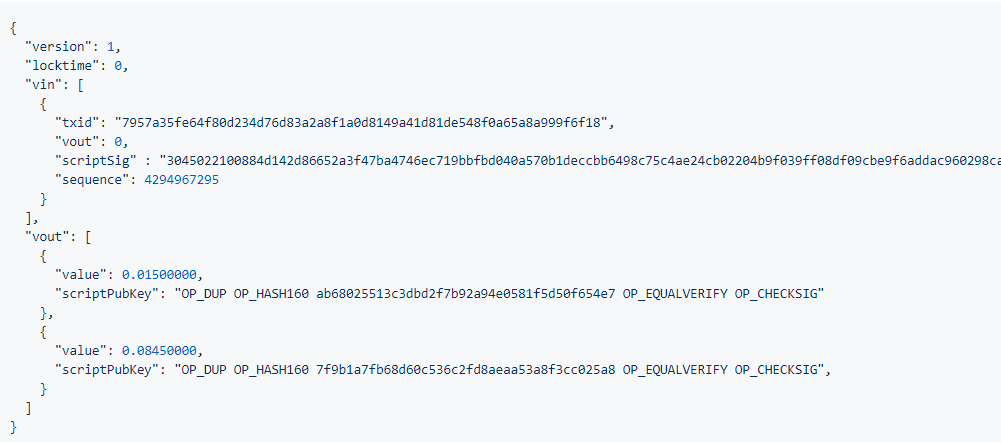
\includegraphics[width=\textwidth]{btc-tx.png}
    \end{center}
    \caption{A decoded Bitcoin transaction~\footcite{https://github.com/bitcoinbook/bitcoinbook/blob/develop/ch06.asciidoc} \label{fig:btc-tx}}
\end{figure}

A transaction is valid if the follwing conditions are fullfilled:

\begin{itemize}
    \item The total value of inputs is greater or equal the total value of outputs.
    \item For all $\varUTXO \opIn \varUTXO$ $\procVerfUTXO{\varUTXO} \opEqNoQ 1$ must hold.
    \item All input UTXOs have not been spent before.
    \item If a locktime $\varTime$ is given, the current block on the Bitcoin blockchain needs to be higher or equal $\varTime$.
\end{itemize}

\begin{definition}[Bitcoin Transaction Scheme]
    We define a Bitcoin Transaction scheme as a tupel of three DPT functions $(\procBuildTransactionId,
    \procSignTransactionId, \procVerfTransactionId)$.
    \begin{itemize}
        \item $\varBtcTx \opFunResult \procBuildTransaction{\varBtcInputs}{\varBtcOutpus}{\varVersion}{\varTime}$: The
        transaction building algorithm is a DPT function which takes as input a set of unspent transaction outputs
        $\varBtcInputs$, a set of newly created transaction outputs $\varBtcOutpus$ a version number $\varVersion$
        and a optional locking time $\varTime$. The algoritm will output an unsigned transaction $\varBtcTx$.
        \item $\funStar{\varBtcTx} \opFunResult \procSignTransaction{\varBtcTx}{\funArray{\varScriptSig}}$: The transaction
        signing algoritm is DPT function which takes as input a unsigned Bitcoin transaction $\varBtcTx$ and an array
        of unlocking scripts $\funArray{\varScriptSig}$ for all inputs of the transaction. The algoritm outputs a
        signed Bitcoin transaction which can now be broadcast to the network.
        \item $\{ 1,0 \} \opFunResult \procVerfTransaction{\varBtcTx}$: The verification algorithm is a DPT function
        taking as input a transaction $\varBtcTx$ outputing 1 on a successfull verification or 0 otherwise. The
        function will check the well-balancedness of the transaction, verify the unlocking scripts, locktime
        as well as scanning through the blockchain if all inputs are indeed unspent.
        Note that any public verifier with access to the blockchain ledger and $\varBtcTx$ will be able to perform the verification.
    \end{itemize}
\end{definition}

Following we will outline two common structures of Bitcoin outputs the P2PK/P2PKH and the P2SH outputs.

\subsubsection{P2PK, P2PKH\label{sec:pre:bitcoin:p2pk}}

P2PK stands for Pay-to-Public-Key and P2PKH for Pay-to-Public-Key-Hash.
In this type of output $\varScriptPubKey$ will be constructed such that its value unlocks if a correct signature is
provided in $\varScriptSig$ for a corresponding public key $\varPubKey$.
P2PKH is an update to this script in which the $\varScriptPubKey$ contains a hashed version of the public key $\varPubKey$,
instead of the public key itself.
To spend a P2PKH output one has to provide the unhashed public key in addition to a valid signature.
This type of output, is the most commonly used output in the Bitcoin blockchain to transfer value from one participant to another.
Delgado et at. found in their paper Analysis of the Bitcoin UTXO set from 2017 that more then 80\% of the UTXO set at
that time consisted of P2PKH transactions, whereas about 17\% were P2SH and 0.12\% P2PK outputs.
~\cite{delgado2018analysis}
P2PKH outputs can be encoded into a Bitcoin address using base58 encoding.
This addresses can be handed out to request a payment from somebody.

\subsubsection{P2SH} \label{sec:pre:bitcoin:p2sh}

If more advanced spending conditions, such as multi signature are required, P2SH (Pay-to-script-hash), introduced in
2012, is a way to implement those in a space efficient and simple matter.
Here the locking condition $\varScriptPubKey$ does not contain a script, but instead the hash of a script.
Upon spending the spender has to provide the original script as well as the unlocking requirements for the script
itself.
Upon verification the hash of the provided script will be computed and compared with the value given in the locking
condition, if those match the actual script will be executed.
The advantages of using this approach over just handcrafting a custom locking script is that the locking scripts are
rather short making the transactions smaller and therefore reducing fees, or rather shifting the fees from the sender
to the owner of the output.
Additionally this type of output can be encoded again into a Bitcoin address similar to a P2PKH output, making it
easy to request a payment.

\section{Privacy-enhancing Cryptocurrencies} \label{sec:pre:privacy}

\subsection{Zero Knowledge Proofs} \label{sec:pre:privacy:zeroknowlegde}

\subsection{Range Proofs} \label{sec:pre:rangeproof}

\begin{definition}[Rangeproof System]
    A Rangeproofs system $\varRProofSystemParam{\varCommitScheme}$ with regards to a homomorphic commitment scheme $\varCommitScheme$ consists of a tupel of functions $(\procRProofSetupId, \procProofId, \procVerfProofId)$.
    \begin{itemize}
        \item $(\varLowerBound,\varUpperBound) \opFunResult \procRProofSetup{\varSecParam}{\varI}{\varJ}$: The rangeproof setup algorithm takes as input a security paramter $\varSecParam$ as well as two numbers
        $\varI$ and $\varJ$ which are treated as exponents of 2 to define the lower and upper bound of the rangeproof protocol.
        \item $\varProof \opFunResult \procProof{\varCommitment}{\varValue}{\varBlindingFactor}$: The proof algorithm is a DPT function which takes as input a commitment $\varCommitment$ a value $\varValue$ and
        a blinding factor $\varBlindingFactor$. It will output a proof $\varProof$ attesting to the statement that the value $\varValue$ of commitment $\varCommitment$ is in between the range $\langle \varLowerBound, \varUpperBound \rangle$ as
        defined during the $\procRProofSetupId$ function.
        \item $\{1,0\} \opFunResult \procVerfProof{\varProof}{\varCommitment}$: The proof verification algorithm is a DPT function which verifies the validity of the proof $\varProof$ with regards to the commitment
        $\varCommitment$. It will output 1 upon a successfull verification or 0 otherwise.
    \end{itemize}
\end{definition}

\begin{definition}[Multiparty Rangeproof System]
    A Multiparty Rangeproof Sytem $\varMPRProofSystemParam{\varCommitScheme}$ with regards to a homomorphic commitment scheme $\varCommitScheme$ is an extension of the regular Rangeproof Sytem with the following
    distributed protocol $\procDRProofId$.
    \begin{itemize}
        \item $\varProof \opFunResult \procDRProof{\varCommitment}{\varValue}{\varBlindingFactorAlice}{\varBlindingFactorBob}$: The distributed proof protocol allows two parties Alice and Bob, each owning a share of the
        commitment $\varCommitment$ to cooperate in order to produce a valid range proof $\varProof$ without a party learning the blinding factor share from the other party.
    \end{itemize}
\end{definition}

For MP proofs \cite{klinec2020privacy}

\section{Mimblewimble} \label{sec:pre:mimblewimble}
In this section we will outline the fundamental properties of the protocols employed in Mimblewimble which are relevant for the thesis and particularily the construction of the Atomic Swap protocol constructed in chapter~\ref{chp:atomicSwap}.
\subsubsection{Transaction Structure} \label{subsec:pre:mimblwimble-tx}

First we will define the notion of a coin in Mimblewimble which has similarity to an unspent transction output (UTXO) in Bitcoin.
\begin{definition}[Mimblewimble Coin]
    For two adjacent elliptic curve generators $\varG$ and $\varH$ a coin in Mimblewimble is a tuple of the form ($\varCoin$, $\varProof$), where $\varCoin \opAssign \funGen{\varValue} \opAddPoint \funGenH{\varNonce}$ is a Pedersen Commitment~\cite{pedersen1991non}
    to the value $\varValue$ with blinding factor $\varNonce$. $\varProof$ is a range proof attesting to the statement that $\varValue$ is in a valid range in zero-knowledge.
    The valid range is defined by the specific implementation, in pratice $\langle 0, 2^{64} -1 \rangle$ is used in the most prominant implementations.
\end{definition}

A Mimblewimble transaction consists of $\varCoinInp \opAssign (\varCoin_1 \opSeperate \dots \opSeperate \varCoin_n)$ input coins and $\varCoinOut \opAssign (\varCoin'_1 \opSeperate \dots \opSeperate \varCoin'_n)$ output coins.
\begin{definition}[Transaction well-balancedness]  \label{def:pre:tx-well-balancedness}
    A transaction is considered \emph{well-balanced} iff $\sum{\varValue'_i} \opSub \sum{\varValue_i} \opEqNoQ 0$ so the sum of all output values subtracted from the sum of input values has to be 0. (Not taking transaction fees into account)
\end{definition}

\begin{definition}[Transaction validity] \label{def:pre:tx-mw-validity}
    A transaction is valid if:
    \begin{itemize}
        \item The transaction is well-balanced as defined in definition~\ref{def:pre:tx-well-balancedness}
        \item $\opForAll \; (\varCoin_i \varProof_i) \opIn \varCoinOut \; \procVerfProof{\varProof_i}{\varCoin_i} \opEqNoQ 1$
    \end{itemize}
\end{definition}

From the definition of \emph{Transaction validity} we can derive the following equation:
\[ \sum{\varCoinOut} \opSub \sum{\varCoinInp} \opEqNoQ \sum{(\funGenH{\varValue'_i} \opAddPoint \funGen{\varNonce'_i})} \opSub \sum{(\funGenH{\varValue_i} \opAddPoint \funGen{\varNonce_i})} \]
So if we assume that a transaction is valid then we are left with the following so called excess value:
\[ \varExcess \opEqNoQ \funGen{\varExcessExp} \opEqNoQ \funGen{(\sum{\varNonce'_i} \opSub \sum{\varNonce_i})} \]
Knowledge of the opening of all coins, and the well-balancedness of the transaction implies knowledge of the discrete logarithm $\varExcessExp$ of $\varExcess$.
Directly revealing $\varExcessExp$ would leak too much information, an adversary knowing the openings for input coins and all but one output coin, could easily calculate the unknown opening given $\varExcess$.
Therefore instead knowledge of the discrete logarithm to $\varExcess$ is proven by providing a valid signature for $\varExcess$ as public key.
Finally we would like to add that coinbase transactions (transactions creating new money as part of mining reward) additionally include the newly minted money as supply $\varSupply$ in the excess equation as follows:
\[ \varExcess \opAssign \funGen{(\sum{\varNonce'_i} \opSub \sum{\varNonce_i})} \opSub \funGenH{\varSupply} \]
Finally a Mimblewimble transaction is of form:
\[ \varTx \opAssign (\varSupply \opSeperate \varCoinInp \opSeperate \varCoinOut \opSeperate \varKernel)\:\text{with}\:\varKernel \opAssign (\funList{\varProof} \opSeperate \funList{\varExcess} \opSeperate \funList{\varSignature}) \]
where $\varSupply$ is the transaction supply amount, $\varCoinInp$ is the list of input coins, $\varCoinOut$ is the list of output coins and $\varKernel$ is the transaction Kernel.
The Kernel consists of $\funList{\varProof}$ which is a set of all output coin range proofs, $\funList{\varExcess}$ a set of excess values and finally $\funList{\varSignature}$ a set of signatures ~\cite{fuchsbauer2019aggregate}.
Even though normally a transaction would only require a single excess value and signature, for reasons we will see in the next section these fields always have to be lists instead of just a single value.

\subsubsection{Transaction Merging \label{sec:pre:mimblewimble:merge}}
An intriging property of the Mimblewimble protocol is that two transactions can easily be merged into a single one, which is essentially a non-interactive version of the CoinJoin protocol on Bitcoin~\cite{maxwell2013coinjoin}.
Assume we have the following two transactions:
\begin{gather*}
    \varTx_0 \opAssign (\varSupply_0 \opSeperate \varCoinInp^0 \opSeperate \varCoinOut^0 \opSeperate (\funList{\varProof_0} \opSeperate \funList{\varExcess_0} \opSeperate \funList{\varSignature_0}) )\\
    \varTx_1 \opAssign (\varSupply_1 \opSeperate \varCoinInp^1 \opSeperate \varCoinOut^1 \opSeperate (\funList{\varProof_1} \opSeperate \funList{\varExcess_1} \opSeperate \funList{\varSignature_1}) )\\
\end{gather*}
Then we can build a single merged transaction:
\[ \varTx_m \opAssign (\varSupply_0 \opAddScalar \varSupply_1 \opSeperate \varCoinInp^0 \opConc \varCoinInp^1,\:\varCoinOut^0 \opConc \varCoinOut^1 \opSeperate (\funList{\varProof_0} \opConc \funList{\varProof_1} \opSeperate
\funList{\varExcess_0} \opConc \funList{\varExcess_1} \opSeperate \funList{\varSignature_0} \opConc \funList{\varSignature_1}) \]
We can easily deduce that if $\varTx_0$ and $\varTx_1$ are valid, it must follow that $\varTx_m$ is valid:\\
If $\varTx_0$ and $\varTx_1$ are valid as of definition~\ref{def:pre:tx-mw-validity} that means $\varCoinInp^0 \opSub \varCoinOut^0 \opSub \funGenH{\varSupply_0} \opEqNoQ \varExcess_0 \opSeperate \funList{\varProof_0}$ contains valid range proofs for the outputs
$\varCoinOut^0$ and $\funList{\varSignature_0}$ contains a valid signature to $\varExcess_0 \opSub \funGenH{\varSupply_0}$ as public key, the same must hold for $\varTx_1$.

By the rules of arithmetic it then must also hold that
\[ \varCoinInp^0 \opConc \varCoinInp^1 \opSub \varCoinOut^0 \opConc \varCoinOut^1 \opSub \funGenH{\varSupply_0 \opAddScalar \varSupply_1} \opEqNoQ \varExcess_0 \opAddPoint \varExcess_1  \]
$\funList{\varProof_0} \opConc \funList{\varProof_1}$ must contain valid range proofs for the output coins and $\funList{\varSignature_0} \opConc \funList{\varSignature_1}$ must contain valid signatures to the respective Excess points, which makes $\varTx_m$ a valid transaction.

\paragraph{Subset Problem} \label{par:pre:mimblewimble:subset}
A subtle problem arises with the way transactions are merged in Mimblewimble.
From the construction shown earlier, it is possible to reconstruct the original separate transactions from a merged one, which can be a privacy issue.
Given a set of inputs, outputs, and kernels, a subset of these will recombine to reconstruct one of the valid transaction which were aggregated since kernel excess values are not combined.
Recall the merged transaction from earlier:
\[ \varTx_m \opAssign (\varSupply_0 \opAddScalar \varSupply_1 \opSeperate \varCoinInp^0 \opConc \varCoinInp^1,\:\varCoinOut^0 \opConc \varCoinOut^1 \opSeperate (\funList{\varProof_0} \opConc \funList{\varProof_1}) \opSeperate
\funList{\varExcess_0} \opConc \funList{\varExcess_1} \opSeperate \funList{\varSignature_0} \opConc \funList{\varSignature_1}) \]
Since the attacker has access to both $\varExcess_0$ and $\varExcess_1$ as well as $\varSignature_0$ and $\varSignature_1$, he can simply try different combinations of input values $\funStar{\funList{\varCoinInp}}$ and output values $\funStar{\funList{\varCoinOut}}$ until he finds a combination under which the transaction is valid with $\varExcess_0, \varSignature_0$ or $\varExcess_1, \varSignature_1$.
Thereby the attacker was able to reconstruct one of the original transactions from which $\varTx_m$ was constructed.
Following this method he might be able to uncover all original transactions from the merged one.

This problem has been mitigated in cryptocurrencies implementing the protocol by including an additional variable $\varOffset$ in the Kernel, called offset value.
Briefly recall the construction of the excess value $\varExcess$:
\[ \varExcess \opAssign \funGen{\varExcessExp} \]
In order to solve the problem we redefine $\varExcess$ as:
\[ \varExcess \opAssign \funGen{\varExcessExp \opSub \varOffset} \]
Since $\varOffset$ is now also included in the transaction kernel and therefore known to the verifier, the public verification is still possible.
Now every time two transactions are merged with the method layed out previously, the two individual offset values $\varOffset_0, \varOffset_1$ are combined into a single value $\varOffset_m$.
If offsets are picked truly randomly, and the possible range of values is broad enough, the probability of recovering the uncombined offsets from a merged one becomes negligible, making it infeasible to recover original transactions from a merged one~\cite{poelstra2016mimblewimble}.


\paragraph{Cut Through} \label{par:pre:mimblewimble:cut}
From the way transactions are merged together, we can now learn how to purge spent outputs securely.
Let's assume $\varCoin_i$ appears as an output in $\varTx_0$ and as an input in $\varTx_1$:
\begin{gather*}
    \varTx_0 \opAssign (\varSupply_0 \opSeperate \varCoinInp^0 \opSeperate \varCoinOut^i \opSeperate (\funList{\varProof_0} \opSeperate \funList{\varExcess_0} \opSeperate \funList{\varSignature_0}) )\\
    \varTx_1 \opAssign (\varSupply_1 \opSeperate \varCoinInp^i \opSeperate \varCoinOut^1 \opSeperate (\funList{\varProof_1} \opSeperate \funList{\varExcess_1} \opSeperate \funList{\varSignature_1}) )\\
\end{gather*}
Essentially this means $\varTx_1$ spends a coin created in $\varTx_0$.
Now lets recall the equation given for transaction well-balancedness in~\ref{def:pre:tx-well-balancedness}:
\[ \sum{\varCoinOut} \opSub \sum{\varCoinInp} \opEqNoQ \sum{(\funGen{\varNonce'_i})} \opSub \sum{(\funGen{\varNonce_i})} \]
If we merge $\varTx_0$ with $\varTx_1$ as done previously the coin $\varCoin_i$ will appear both in $\sum{\varCoinInp}$ and $\sum{\varCoinOut}$.
Therefore we can erase $\varCoin_i$ from both lists, while maintaining transaction balancedness.
Informally this means that every time a coin gets spend, it can be erased from the ledger, without breaking the rules of the system.
This property is employed in the Mimblewimble protocol to reduce the space requirements of the protocol as well as provide a notion of unlinkability, as transaction histories can be erased.

\subsubsection{Transaction Building} \label{subsec:pre:mimblewimble:txbuild}
As already pointed out, building transactions in Mimblewimble is an interactive process between the sender and receiver of funds.
Jedusor, Tom Elvis originally envisioned the following two-step process to build a transaction:~\cite{jedusor2016mimblewimble}

Assume Alice wants to transfer coins of value $\varFundValue$ to Bob.
\begin{enumerate}
    \item Alice first selects an input coin $\varCoinInp$ (or potentially multiple) in her control with total stored value $\varValue$ with $\varValue \geq \varFundValue$.
    She then creates change coin outputs $\varCoinOutAlice$ (could again be multiple) with the remainder of her input value substracted by the value send to Bob.
    For her newly created output coins and her input coins she calculates her part of discrete logarithm $\varKey$ (her part of the key) to the final $\varExcess$ and sends all this information to Bob as a pre-transaction.
    \item Bob creates himself additional output coins $\varCoinOut^B$ of total value $\varFundValue$ and similar to Alice creates his share $\funStar{\varKey}$ of the discrete logarithm of $\varExcess$.
    Together with the share received by Alice he can now create a signature to $\varExcess$ and finalize the transaction
\end{enumerate}
Figure~\ref{fig:txOriginal} depicts the original transaction flow.\\
\begin{figure}
    \centering
    \pseudocode[codesize=\scriptsize]{
        \textbf{Alice} \< \< \< \< \textbf{Bob} \\ [][\hline]
        \< \< \< \< \\
        \text{ Select $\varCoinInp$ of value $\varValue \geq \varFundValue$ } \< \< \< \< \\
        \text{ Create $\varCoinOutAlice$ of value $\varValue \opSub \varFundValue$} \< \< \< \< \\
        \text{ $\varExcess_{A} \opAssign \sum{\varCoinOutAlice} \opSub \sum{\varCoinInp}$ } \\
        \text{ $(-\varFundValue \opSeperate \varKey)$ opening to $\varExcess_{A}$ } \< \< \< \< \\
        \text{ Create range-proof $\varProof$ for $\varCoinOutAlice$ } \< \< \< \< \\
        \< \sendmessageright{ top=$(-\varFundValue \opSeperate \varKey) \opSeperate \varProof$ } \< \< \< \\
        \< \< \< \< \text{Create $\varCoinOut^B$ with value $\varFundValue$ and keys $(\varKeySt_i)$ } \\
        \< \< \< \< \text{$\varKey_{shared} \opAssign \varKey \opAddScalar \sum{\varKeySt_i}$ } \\
        \< \< \< \< \text{Create $\varSignature$ with $\varKey_{shared}$} \\
        \< \< \< \< \text{ Create range-proof $\varProof$ for $\varCoinOutBob$ } \\
        \< \< \< \< \text{Finalize transaction $\varTx$} \\
    }
    \caption{Original transaction building process\label{fig:txOriginal}}
\end{figure}

This protocol however turned out to be insecure as it is vulnerable to the following attack:
The receiver could spend Alice's change coins $\varCoinOut^A$ by reverting the transaction.
Doing this would give the sender his coins back, however as the sender might not have the keys for his spent outputs anymore, the coins could then be lost.

In detail this reverting transaction would look like:
\[ \varTx_{rv} \opAssign (0 \opSeperate \varCoinOut^A \opConc \varCoinOut^B \opSeperate \varCoinInp \opSeperate (\varProof_{rv} \opSeperate \varExcess_{rv} \opSeperate \varSignature_{rv}) ) \]
So in essence it is exactly the reverse of the previous transaction.
Again remembering the construction of the excess value of this construction would look like this:
\[ \varExcess_{rv} \opAssign \sum{\varCoinOut^A \opConc \varCoinOut^B \opSub \varCoinInp} \]
The key $\varKey$ originally sent by Alice to Bob is a valid opening to $\sum{\varCoinInp} \opSub \sum{\varCoinOut^A}$. With the inverse of this key $\varKey_{inv}$ we get the opening to $\sum{\varCoinOut^A \opSub \varCoinInp}$.
Now all Bob has to do is add his key $\funStar{\varKey}$ to get:
\[ \varKey_{rv} \opAssign -\varKey \opAddScalar \funStar{\varKey} \]
which is the opening to $\varExcess_{rv}$.
Therefore Bob is able to construct a valid signature under $\varExcess_{rv}$.
Range proofs can just be reused, because this transaction spends to a coin which has already existed on the ledger with the same blinding factor and value, meaning the proof will still be valid.

In essence this means Bob spends the newly created outputs and sends them back to the original input coins, chosen by Alice. It might at first seem unclear why Bob would do that.
An example situation could be if Alice pays Bob for some good which Bob is selling. Alice decides to pay in advance, but then Bob discovers that he is already out of stock of the good that Alice ordered.
To return the funds to Alice, he reverses the transaction instead of participating in another interactive process to build a new transaction with new outputs.
If Alice already deleted the keys to her initial coins, the funds are now lost.
The problem was solved in the Grin and Beam Mimblewimble implementations by making the signing process itself a two-party process which will be explained in more detail in chapter~\ref{chp:fixedWitnessSignatures}.

Alternatively Fuchsbauer et al.~\cite{fuchsbauer2019aggregate} proposed another way to build transactions which would not be vulnerable to this problem:
\begin{enumerate}
    \item Alice constructs a full-fledged transaction $\varTx_A$ spending her input coins $\varCoinInp$ and creates her change coins $\varCoinOut^A$, plus a special output coin $\varCoinSpecial \opAssign \funGenH{\varFundValue} \opAddPoint \funGen{\varKey_{sp}}$,
    where $\varFundValue$ is the desired value which should be transferred to Bob and $\varKey_{sp}$ is a randomly choosen key. She proceeds by sending $\varTx_A$ as well as $(\varFundValue \opSeperate \varKey_{sp})$ and the necessary range
    proofs to Bob.
    \item Bob now creates a second transaction $\varTx_B$ spending the special coin $\varCoinSpecial$ to create an output only he controls $\varCoinOutBob$ and merges $\varTx_A$ with $\varTx_B$
    into $\varTx_m$. He then broadcasts $\varTx_m$ to the network. Note that when the two transactions are merged the intermediate special coin $\varCoinSpecial$ will be both in the coin output and input list
    of the transaction and therfore will be discarded.
\end{enumerate}
One drawback of this approach is that we have two transaction kernels instead of just one because of the merging step, making the transaction slightly bigger, however there is still only one interaction required between Alice and Bob.
In the solution employed by the Grin and Beam implementations which we will discuss in chapter~\ref{chp:atomicSwap}, at least one additional round of interaction will be required.
A figure showing the protocol flow is depicted in Figure~\ref{fig:txSalvaged}.

\begin{figure}
    \centering
    \pseudocode[codesize=\scriptsize]{
        \textbf{Alice} \< \< \< \< \textbf{Bob} \\ [][\hline]
        \< \< \< \< \\
        \text{ Select $\varCoinInp$ of value $\varValue \geq \varFundValue$ } \< \< \< \< \\
        \text{ Create $\varCoinOutAlice$ of value $\varValue \opSub \varFundValue$ } \< \< \< \< \\
        \varKey_{sp} \sample \cnstIntegersPrimeWithoutZero{\varPrime} \< \< \< \< \\
        \text{ Create $\varCoinSpecial \opAssign \funGenH{\varFundValue} \opAddScalar \funGen{\varKey_{sp}}$ } \< \< \< \< \\
        \text{ Construct and sign $\varTxAlice$ with $\varCoinInp \opSeperate \varCoinOutAlice \opSeperate \varCoinSpecial$ } \< \< \< \< \\
        \< \sendmessageright{ top=$\varTxAlice \opSeperate \varFundValue \opSeperate \varKey_{sp}$ } \< \< \< \\
        \< \< \< \< \text{ Create $\varCoinOut^B$ with value $\varFundValue$ } \\
        \< \< \< \< \text{ Create $\varTxBob$ spending $\varCoinSpecial$ to $\varCoinOut^B$ } \\
        \< \< \< \< \text{ Merge $\varTxAlice$ and $\varTxBob$ to $\varTx_{m}$ } \\
        \< \< \< \< \text{ Publish $\varTx_{m}$ }
    }
    \caption{Salvaged transaction protocol by Fuchsbauer et al.~\cite{fuchsbauer2019aggregate} \label{fig:txSalvaged}}
\end{figure}

\section{Scriptless Scripts} \label{sec:pre:scriptless-scripts}

\section{Adaptor Signatures} \label{sec:pre:aptsignatures}

